\documentclass[10pt,twocolumn]{article}

\usepackage[margin=0.85in]{geometry}
\usepackage{amsmath}
\usepackage{amssymb}
\usepackage{graphicx}
\usepackage{booktabs}
\usepackage{xcolor}
\usepackage{listings}
\usepackage{url}
\usepackage[hidelinks]{hyperref}
\usepackage{caption}
\usepackage{subcaption}

\definecolor{cgreen}{RGB}{27,120,55}
\definecolor{cred}{RGB}{178,24,43}
\definecolor{camber}{RGB}{191,129,45}

\newcommand{\green}[1]{\textcolor{cgreen}{\textsc{#1}}}
\newcommand{\amber}[1]{\textcolor{camber}{\textsc{#1}}}
\newcommand{\red}[1]{\textcolor{cred}{\textsc{#1}}}
\newcommand{\tool}{\textsc{EmitRust}}
\newcommand{\ie}{i.e.\ }
\newcommand{\eg}{e.g.\ }

\lstset{
  basicstyle=\ttfamily\scriptsize,
  columns=fullflexible,
  keepspaces=true,
  breaklines=true,
  frame=leftline,
  framesep=4pt,
  xleftmargin=6pt,
  aboveskip=6pt,
  belowskip=4pt,
}

\title{\vspace{-2em}Compiling Partial Translations:\\
Emission-Derived Dependency Colouring and\\
Directionally-Unsound Approximation for\\
Incremental C\texttt{++}-to-Rust Migration}

\author{}
\date{}

\begin{document}
\maketitle

\begin{abstract}
Source-to-source translators from C/C\texttt{++} to Rust are conventionally
all-or-nothing: a single construct outside the supported subset causes the
whole translation unit---in a multi-file project, the whole project---to be
rejected, so a large real codebase yields no output at all until the
translator is complete. We describe a system in which the unit of output is
instead a \emph{compiling partial crate}: every program item the translator
can handle is emitted as real Rust, every item it cannot is emitted as a
signature-preserving stub or dropped, and the resulting crate is required to
build. Progress is then a measurable quantity---the fraction of program items
translated---rather than a binary.

Making this work required three design decisions that we believe are not
obvious, and which we argue generalise beyond this system. First, the
dependency graph over program items must be \emph{kinded by the emission
contract of the target language}, not by the dependency structure of the
source: whether a missing dependency poisons its dependent is decided by
whether the generated Rust textually \emph{spells} that dependency, which
makes an otherwise-identical C construct poisoning or benign according to how
the backend renders it. Second, a static approximation that feeds a
\emph{subtractive} repair search must be deliberately unsound \emph{in one
direction}: because the search can only withdraw items and never re-admit
them, a false negative is an unrecoverable loss while a false positive costs
one probe, so the approximation must be tuned to never under-admit. Third,
the trivial solution must be a member of the search space, which turns
``optimisation never makes the result worse'' from a property one hopes for
into one that holds structurally.

We evaluate on 352 projects---six C\texttt{++} projects, thirteen C programs,
and two regression corpora---comprising 1337 program items. Partial
translation raises the projects yielding a compiling Rust crate from 338 to
349 of 352, with the gain concentrated where it should be: $4/6 \rightarrow
6/6$ on the C\texttt{++} projects and $9/13 \rightarrow 13/13$ on the C
programs, against no movement on a regression corpus already inside the
subset. On a separate 18-project benchmark held fixed across eight revisions
of the translator, with an all-or-nothing control series that isolates the
mode from growth of the supported subset, the count rises from 11 to 18 while
the control reaches only 12, and no revision ever emits a crate that fails to
build.

The colouring commits zero false negatives across all 1337 items, as its
contract requires. Three results qualify the design, and we report them
because each cost us a claim we had already written down. The repair search
improves 3 of 352 projects and regresses none---but all three are fixtures we
wrote to exercise it, so on non-synthetic input it improves nothing; an
earlier version of this evaluation reported nine improvements, six of which
turned out to be our own harness feeding multi-unit projects half their
source. A budget sweep shows our shipped search bound is four times larger
than any project needs. The middle value of our three-valued lattice is never assigned
by any project we measured. And we report a blind spot our own benchmark had
designed into it: library projects were unreachable under any flag, and no
program in the corpus could reveal it, because every one had been written with
an entry point so the differential oracle would have something to run.
\end{abstract}

\section{Introduction}
\label{sec:intro}

The practical obstacle to migrating a C or C\texttt{++} codebase to Rust is
not that translation is impossible but that it is incomplete. Every
source-to-source translator supports a subset of the input language, and every
real codebase contains constructs outside it. The conventional response is to
reject: the translator emits a diagnostic and stops, and the engineer sees
nothing. The consequence is that the translator delivers zero value until it
is nearly complete, and that ``how far along are we'' has no answer beyond a
list of error messages.

This paper describes the alternative we built into \tool{}, an MLIR-based
C/C\texttt{++}-to-Rust translator. The output of a translation is a Rust crate
that \emph{compiles}, containing real translations of the items the tool
handles and stubs for the items it does not, together with a per-item
accounting of what happened and why. A project entirely outside the supported
subset still produces a buildable skeleton; a project partly inside produces a
crate a developer can immediately compile, test, and finish by hand.

The engineering to get there is mostly unremarkable. Three decisions are not,
and they are the contribution of this paper.

\paragraph{Contribution 1: emission-derived dependency semantics
(\S\ref{sec:colouring}).} We build a dependency graph over program items
(functions, records, enums, globals) and propagate a three-valued colour over
it. The non-obvious part is what the edges mean. Whether a missing dependency
poisons its dependent is not a property of the C dependency---it is a property
of \emph{how the backend renders that dependency in Rust}. A function whose
callee is missing can still be emitted, because Rust lets one write a
type-correct body-less function; a record whose field type is missing cannot,
because the field list must name the type. The same distinction cuts
\emph{within} a single edge kind: a by-value field spells its type in the
generated struct and therefore poisons, while a pointer field is erased to an
integer handle by our pointer model and therefore does not. Edge kind is thus
a function of the code generator, and a change to the generator is a change to
the graph.

\paragraph{Contribution 2: directional unsoundness for subtractive search
(\S\ref{sec:search}).} A static admissibility probe seeds the colouring; a
bounded search then repairs the probe's mistakes by attempting a real
translation and withdrawing items that fail. Because the search is
\emph{subtractive}---it removes items from the admitted set and never adds
them---the two error directions have radically different costs. A false
positive (an item admitted that turns out to fail) costs one translation
probe. A false negative (an item excluded that would have succeeded) is
\emph{unrecoverable}: nothing in the system can put it back. The approximation
must therefore be deliberately, asymmetrically unsound, and we state this as a
design rule with a measured justification.

\paragraph{Contribution 3: the trivial solution as a search state
(\S\ref{sec:baseline}).} A repair search that can reduce the admitted set can,
if its seed is wrong, produce a worse result than not searching at all---and
in our system it did, until we found it. The fix is structural rather than
defensive: the unrestricted translation is itself a point in the search space,
so the search evaluates it like any other candidate and takes the maximum.
``Search never loses to no search'' then follows from the definition of a
maximum rather than from a test.

\paragraph{Contribution 4: progress as a measured quantity
(\S\ref{sec:progress}).} Because every project yields a compiling artifact
with per-item status, the state of the translator against a benchmark is a
number. We ratchet it, attribute each unported item to a \emph{root cause}
rather than to the symptom it presents, and use the resulting ranked backlog
to sequence development. \S\ref{sec:eval} shows this loop operating across
eight revisions.

We are explicit about what we do not claim. The search component's value is
corpus-dependent in a way we can characterise but not generalise:
\S\ref{sec:eval-search} shows it converting eight total failures into partial
successes while changing nothing on our four-project C\texttt{++} benchmark,
and explains both in terms of Contribution 2. We do
not claim the translated subset is large; it is not. We claim that the
\emph{shape} of the output---always compiling, always accounted for---changes
what a partial translator is worth, and that the three design rules above are
what make that shape achievable.

\section{Background and Motivation}
\label{sec:background}

\tool{} translates a subset of C99 and a smaller subset of C\texttt{++}
through an MLIR dialect to safe Rust. Its soundness argument is
\emph{differential}: a translated program is accepted only when the emitted
crate builds and its observable output matches, byte for byte, a native build
of the same sources by a reference C/C\texttt{++} compiler. This choice
matters for what follows, and we contrast it with verification-condition
approaches in \S\ref{sec:related}.

The pipeline's relevant property is that translation is a \emph{whole-project}
operation with a single failure mode. Sources are parsed as independent
translation units and merged into one module with cross-unit symbol
resolution; the merged module is lowered and emitted. Before the work
described here, the top-level declaration walk returned failure at the first
declaration it could not handle, and both the single-file and whole-project
entry points propagated that failure. One unsupported construct anywhere
therefore produced no output at all---the precise reason a real C\texttt{++}
project yielded nothing.

\subsection{Why partiality is not simply ``skip it''}
\label{sec:why-hard}

The naive fix---skip declarations that fail and emit the rest---does not
produce a compiling crate, for three reasons that motivate the rest of the
paper.

\emph{Dangling references.} A skipped item may be named by an item that
succeeded. A dropped record referenced by a surviving function signature
yields Rust that does not compile. Something must propagate the loss.

\emph{Partial state.} A declaration that fails midway has already mutated the
translator's state---emitted operations, claimed symbol names, populated
analysis caches. Resuming requires the failed item to leave no trace, which is
a stronger requirement than reporting an error and exiting.

\emph{Asymmetric substitutability.} Some losses can be papered over and others
cannot, and which is which is a property of Rust, not of C. This is
Contribution 1, and we develop it next.

\section{Emission-Derived Dependency Colouring}
\label{sec:colouring}

\subsection{The item graph}

We construct a graph whose nodes are \emph{program items}---the things the
translator emits as top-level Rust items---and whose edges are kinded
dependencies. Node keys are the emitted Rust symbol names, produced by calling
the same naming functions the translator itself calls, so that a graph node
and an emitted item are the same object by construction rather than by
convention. The graph is built by a pure analysis over the parsed ASTs, with
no IR construction, so it is available for projects the translator cannot
translate---which is the point, since those are exactly the projects whose
dependency structure one wants to inspect.

Edge kinds are listed in Table~\ref{tab:edges}. The graph is \emph{closed}: an
edge is recorded only when both endpoints are nodes, so a consumer never has
to resolve a dangling target.

\begin{table}[t]
\centering
\footnotesize
\caption{Edge kinds of the item graph. The rightmost column is the
propagation strength derived in \S\ref{sec:colouring}: whether a \red{red}
target poisons its source \red{red}, only demotes it to \amber{yellow}
(because the target is stub-replaceable), or does not poison it at all
(because the emitted Rust never names the target).}
\label{tab:edges}
\begin{tabular}{@{}llc@{}}
\toprule
\textbf{Edge} & \textbf{Meaning} & \textbf{Poison} \\
\midrule
\textsc{Calls}          & body calls the target        & \amber{yellow} \\
\textsc{CallsIndirect}  & call through a fn pointer    & --- \\
\textsc{SigType}        & type named in the signature  & \red{red} \\
\textsc{BodyType}       & type named inside the body   & \red{red}$^\dagger$ \\
\textsc{Field}          & field spells the type        & \red{red} \\
\textsc{FieldIndirect}  & field reaches it via pointer & none \\
\textsc{Base}           & C\texttt{++} base class      & \red{red}$^\ddagger$ \\
\textsc{ReadsGlobal}    & body reads the global        & \red{red} \\
\textsc{WritesGlobal}   & body writes the global       & \red{red} \\
\textsc{TakesAddressOf} & address of a function        & \amber{yellow} \\
\bottomrule
\end{tabular}

\vspace{2pt}
\raggedright\scriptsize
$^\dagger$ Poisons the function \red{red}, but the function stays
stub-replaceable, so its own callers are only \amber{yellow}
(\S\ref{sec:colouring}).\\
$^\ddagger$ Vacuous in practice: a record with a direct base is already an
inadmissible seed, so a \textsc{Base} edge never decides a colour. Retained
for totality.\\
\textsc{CallsIndirect} carries no target and so cannot propagate; it is
recorded because ``this item makes an indirect call'' is itself the fact a
port-order consumer needs.
\end{table}


\subsection{The colouring lattice}

Over this graph we compute a least fixed point assigning each item one of
three colours:

\begin{itemize}
\item \green{green}: the item and its entire type closure are inside the
supported subset;
\item \amber{yellow}: the item itself is admissible, but some dependency is
\red{red}---it will be emitted, calling a stub;
\item \red{red}: the item is itself inadmissible, or a dependency it cannot
survive the loss of is \red{red}.
\end{itemize}

The lattice is seeded by a syntactic admissibility probe over the AST---a
screen for constructs the translator rejects by construction (templates,
virtual methods, base classes, exceptions, and so on).

\subsection{The rule, and why it is not per-edge}

Our first formulation had one propagation rule per edge kind, and it was
wrong. The correct formulation is a single rule:

\begin{quote}
An edge to a \red{red} target poisons its source \red{red}, \emph{unless the
target is stub-replaceable}, in which case the source is only \amber{yellow}.
\end{quote}

\noindent where \emph{stub-replaceable} is quoted directly from the recovery
policy of the emitter: a rejected function whose signature still maps is
replaced by a stub carrying that signature; everything else is dropped. The
entire lattice is therefore determined by one property of the target language:
\textbf{Rust lets you write a function with a correct signature and no
meaningful body, and does not let you write a type with a correct name and no
definition.} A missing function is substitutable; a missing type is not.

Three consequences follow, none of which we anticipated when we specified the
system, and each of which we had to be corrected on by the implementation:

\paragraph{Body dependencies poison, but stop at the function boundary.} A
record used only inside a function body poisons that function \red{red}---the
statements mentioning it cannot be written. But the function's \emph{signature}
never named the record, so the function remains stub-replaceable and its own
callers are merely \amber{yellow}. Red bodies stop exactly where a stub can be
inserted.

\paragraph{Signature dependencies poison \emph{and} remove
substitutability.} A function whose parameter type is \red{red} cannot be
stubbed, because the stub's own parameter list would have to name the missing
type. Its callers are therefore \red{red}, not \amber{yellow}. This is the
case our original specification got wrong: we had assumed call-edge poisoning
always yields \amber{yellow}.

\paragraph{Unsubstitutability does not propagate; only redness does.} A caller
of a signature-broken function is \red{red} but is \emph{itself}
stub-replaceable, so \emph{its} caller is \amber{yellow}. Without this rule a
single unsupported type reddens an entire program; with it, damage is confined
to a radius of one stub boundary.

\subsection{The same edge kind, two semantics}
\label{sec:field-indirect}

The sharpest illustration that edge semantics come from the emitter, not the
source, is the field edge. Consider two C records, identical but for one
pointer:

\begin{lstlisting}
struct Holder  { struct Atom  a; int k; };
struct HolderP { struct Atom *p; int k; };
\end{lstlisting}

Both depend on \texttt{struct Atom} in the source language. In the generated
Rust they do not. The by-value field renders as \texttt{a: Atom} and names the
type; the pointer field is erased by our pointer model to an integer handle
and names nothing. If \texttt{Atom} is dropped, the first crate fails to
compile and the second compiles unchanged.

The dependency graph must therefore distinguish them, and we introduce a
distinct edge kind---\textsc{FieldIndirect}---for the erased case. The
governing rule is: \textbf{a field edge poisons if and only if the emitted
Rust spells the target.} Table~\ref{tab:field} gives the cases we verified
empirically rather than by inspection.

\begin{table}[t]
\centering
\footnotesize
\caption{The field-edge rule, established empirically: a field edge poisons
if and only if the emitted Rust \emph{spells} the target's name. Each row was
verified by dropping \texttt{struct Atom} and asking whether the emitted crate
compiles---not by reasoning about the C type system, in which every row is a
dependency.}
\label{tab:field}
\begin{tabular}{@{}llcl@{}}
\toprule
\textbf{C field} & \textbf{emitted Rust} & \textbf{builds} & \textbf{edge} \\
\midrule
\texttt{struct Atom a}       & \texttt{a: Atom}     & no  & \textsc{Field} \\
\texttt{struct Atom a[3]}    & \texttt{[Atom; 3]}   & no  & \textsc{Field} \\
\texttt{int (*f)(struct Atom)} & prototype names it & no  & \textsc{Field} \\
\texttt{struct Atom *p}      & \texttt{p: i64}      & yes & \textsc{FieldIndirect} \\
\texttt{struct Atom **pp}    & erased               & yes & \textsc{FieldIndirect} \\
\texttt{struct Atom *a[4]}   & erased               & yes & \textsc{FieldIndirect} \\
\bottomrule
\end{tabular}

\vspace{2pt}
\raggedright\scriptsize
The function-pointer row is the instructive one: the field crosses a pointer,
yet the prototype still spells \texttt{Atom}, so it poisons. Pointer-ness is
not the criterion; \emph{appearing in the generated text} is.
\end{table}


We stress the methodological point. We did not derive this table from the C
type system; we derived it by generating both crates, dropping the target, and
asking \texttt{rustc}. The same procedure applied to signature edges confirmed
they are exact---a \texttt{struct Atom *} \emph{parameter} renders as
\texttt{\&mut Atom} and \emph{does} name the record, so no pointer exemption
exists there---and showed the base-class edge to be vacuous, since any record
with a base is already an inadmissible seed. An analysis whose edge semantics
track a code generator can only be validated against that code generator.

\section{Recoverable Translation}
\label{sec:recovery}

Recovery mode records a rejected top-level item in a ledger---symbol, source
location, verbatim diagnostic, blocker tag---and continues the declaration
walk. A rejected function whose signature still maps is emitted as a stub with
that signature and an \texttt{unimplemented!()} body; anything else is dropped,
and items depending on it fail in turn and are recovered by the same
mechanism, which is the colouring's prediction observed dynamically.

Two aspects are worth reporting.

\paragraph{Rollback.} A declaration that fails midway must leave no trace. We
checkpoint the module body and undo: erase operations appended past the
checkpoint, roll back the symbol tables that named them, and reset the
per-function analysis state whose values point into erased regions. We
deliberately do \emph{not} roll back records, enums, and globals that the
failed item pulled in on demand: their name registries have no inverse, and
erasing the operation while retaining the registry entry would leave a
dangling symbol, which is worse than a dead one that the crate's
\texttt{allow(dead\_code)} already covers. The cost is that a recovered crate
may carry unused definitions. We state this rather than hide it because it is
the kind of asymmetry---dead is recoverable, dangling is not---that recurs
throughout this design.

\paragraph{A cascade bug the invariant exposed.} Our first implementation
marked a record as imported \emph{before} walking its fields, so a record that
was subsequently rejected still returned an emitted name, and uses of it built
a type referring to a struct nobody defined. The resulting crate reported a
higher ported count and did not compile. This is precisely the failure the
colouring predicts and the ``crate must build'' invariant is designed to
catch; it was invisible to any test that only checked the translator's own
exit code. We discuss its effect on our measurements in
\S\ref{sec:eval-yield}.

\section{Subtractive Repair Search}
\label{sec:search}

The admissibility probe is syntactic and therefore imprecise. A bounded
best-first search repairs it. A search state is a set of admitted items; the
score is lexicographic in (items emitted for real, negated stub count,
representation cost); expansion probes a state by running a recovering
translation and, for each rejection reported, generates a child state with the
offending item withdrawn.

\subsection{Why the probe must be unsound in one direction}
\label{sec:directional}

The search is \emph{subtractive}: children are always proper subsets of their
parent. Nothing in the system re-admits an item the seed excluded. Therefore:

\begin{itemize}
\item A \textbf{false positive}---the probe calls an item admissible and the
translation rejects it---costs \emph{one probe}. The search observes the
rejection, withdraws the item, and converges.
\item A \textbf{false negative}---the probe calls an item inadmissible when the
translation would have accepted it---is \textbf{unrecoverable}. The item is
never in any admitted set, and no amount of search budget recovers it.
\end{itemize}

The design rule follows directly, and we state it as the paper's most
transferable claim:

\begin{quote}
\emph{An approximation that seeds a subtractive search must be tuned to
minimise false negatives even at substantial cost in false positives. When in
doubt, admit.}
\end{quote}

This inverts the usual instinct in static analysis, where soundness means
over-approximating the set of bad things. Here the analysis is a
\emph{scheduling hint} for a search that can verify, and the verifier's
existence is what licenses---indeed requires---unsoundness in the permissive
direction. Our probe accordingly declines to screen several constructs it
could screen syntactically, because whether they translate depends on facts
the syntax does not determine.

\subsection{The trivial solution as a state}
\label{sec:baseline}

Directional unsoundness is a discipline, and disciplines fail. We therefore
enforce the consequence structurally. The unrestricted recovering
translation---the state admitting every item---is itself a point in the search
space. The search probes it unconditionally and scores it by the same rule.
Since the returned result is a maximum over probed states, and the
unrestricted translation is always one of them:

\[
\mathrm{score}(\text{search}) \;\ge\; \mathrm{score}(\text{no search})
\]

\noindent holds by the definition of a maximum, not by testing. A colouring
bug can then cost search time but cannot cost translated items. We
additionally check the inequality at run time and fall back if it is ever
violated, because the assertion that states it is compiled out of release
builds---the configuration in which users rely on the guarantee.

We arrived at this only after observing the failure. An earlier revision
produced a \emph{lower} ported count with search enabled than without it,
which is the pathology this construction eliminates.

\section{Progress as a Measured Quantity}
\label{sec:progress}

\subsection{Root-cause attribution}

Every unported item carries a direct blocker---the tag of the diagnostic
actually raised. Direct blockers are a poor work list, because most of them
are cascades. In one of our benchmarks, thirteen items report the identical
diagnostic ``method of an unimported class''; all thirteen are consequences of
one destructor and three base classes. A developer reading the direct tally
sees thirteen symptoms and no causes.

The colouring already computes what is needed: for each non-green item, the
chain of poison edges terminating at an inadmissible root, and that root's
construct tag. Attribution joins the chain into the report, so items are
ranked by \emph{root} cause while the direct tally is retained. The
compression this achieves is measured in \S\ref{sec:eval-attrib}.

Attribution must handle items the graph does not model---C\texttt{++} member
functions are not graph nodes, yet they are exactly the thirteen symptoms
above. We attribute a method to its enclosing class's node, recording the
owner at rejection time rather than recovering it from the symbol, since
nothing in a mangled method name identifies its class and sibling classes
define identically-named methods.

\subsection{Ratcheting}

Per-item status is recorded in a per-project manifest and checked two ways: a
regression fails the build, an improvement fails until ratcheted forward
explicitly. Development is then an optimisation loop against a fixed
benchmark, and \S\ref{sec:eval-long} plots it.

\section{Experimental Design}
\label{sec:expdesign}

We ask five questions.

\begin{description}
\item[E1] How precise is the colouring against ground truth, and---critically
for \S\ref{sec:directional}---is the false-negative rate actually zero?
\item[E2] What fraction of projects yields a \emph{compiling} artifact under
all-or-nothing translation versus partial translation, and what fraction of
program items is translated?
\item[E3] What does the repair search cost, and what does it buy?
\item[E4] Does translated-item fraction increase monotonically across
successive revisions of the translator, on a fixed benchmark?
\item[E5] By how much does root-cause attribution compress a work list?
\item[E6] What do the pure-AST analyses cost relative to translation?
\end{description}

\paragraph{Benchmarks.} Four C\texttt{++} projects of several translation units
each, spanning a deliberate difficulty gradient from near-in-subset to
solidly-outside; thirteen self-contained C programs; and two single-file
regression corpora. The C\texttt{++} projects are the demand-signal corpus: they
are not expected to translate completely, and their purpose is to generate
ranked blockers.

\paragraph{Ground truth for E1.} The colouring predicts; the recovering
translation decides. We join predicted colour against realised per-item status
on the shared symbol key. A \emph{false green} is an item predicted
green/yellow that was dropped; a \emph{false red} is an item predicted red
that was ported. Only the latter is a contract violation.

\paragraph{Methodology for E4.} The benchmark must be held fixed while the
tool varies. Since the corpus itself was introduced and ratcheted during the
period measured, we extract the corpus once from the newest revision and run
every historical build of the translator against \emph{that} fixed copy. Two
series are reported, because capability differs across the range: artifact
yield is defined at every revision, while per-item fraction is defined only
from the revision that introduced per-item accounting.

\paragraph{Threats.} Our benchmark is small and authored by us, which bounds
external validity; we report per-project numbers rather than only aggregates
so the reader can judge. Timings are wall-clock best-of-three on a deliberately
non-quiescent 20-core machine---a desktop session, container workloads, and
concurrent builds were running throughout, with load averages of 3.5--11.0. A
best-of-five recheck on a 25-project subset agrees within 10\,\%. Mode-to-mode
\emph{ratios} are measured back to back and are trustworthy; absolute
milliseconds, especially \texttt{cargo} times, should be read as upper bounds.
We also cannot isolate the clang parse cost, because no mode of the tool
parses and stops; \S\ref{sec:eval-cost}'s parse-dominance claim rests on the
scaling argument, not on a direct measurement of the parse. E1's ground
truth is the translator's own behaviour, so it measures the colouring's
agreement with the emitter, not with an independent oracle---which is the
correct target, since the colouring exists to predict the emitter.

\section{Results}
\label{sec:eval}

\subsection{E1: colouring precision}
\label{sec:eval-precision}

We measured 1337 program items across 344 projects in four corpora
(Table~\ref{tab:e1}, Figure~\ref{fig:e1}). No project was excluded: every one
produced a per-item report.

\paragraph{The contract holds.} There are \textbf{zero false negatives} in the
entire measured set: no item the colouring called \red{red} was subsequently
translated. This is the property \S\ref{sec:directional} argues is
non-negotiable, and it is the one we can only establish empirically---we do
not prove it, and one deliberately-retained source of false negatives survives
in the implementation (\S\ref{sec:discussion}), recovered by the construction
of \S\ref{sec:baseline} rather than by the probe.

\paragraph{False positives are rare and cheap.} Two items across 1337 were
admitted and then dropped ($0.15\,\%$). At that rate the search's repair role
is nearly idle, which is precisely what \S\ref{sec:eval-search} goes on to
measure. One of the three is instructive about measurement itself: it is the
\texttt{main} of a program that, until the revision described in
\S\ref{sec:discussion}, produced no report at all. The probe's judgement on it
was always wrong; the item had simply never been \emph{scorable} before. A
previously unmeasurable miss is not a new miss, and the difference matters
when reading any precision figure.

\paragraph{An unexercised lattice value.} The \amber{yellow} state---an item
that is itself admissible but calls something that is not---was assigned to
\textbf{no item in any corpus}. This is a genuine negative result about our
benchmark rather than about the design. \amber{yellow} requires a project in
which a translatable function calls an untranslatable one whose signature
still maps; our C\texttt{++} projects instead fail at types (references,
bases, destructors), which poison \red{red} directly, and our C corpora barely
fail at all. The state is load-bearing in the rule---removing it would
collapse call-poisoning into type-poisoning and redden whole programs---but
we cannot claim benchmark support for it, and we flag the gap rather than
quietly reporting a three-valued lattice that behaves as a two-valued one
here.

% Nine columns do not fit a single column at 10pt, so this one spans
% both. Kept as generated output rather than hand-tuned in the source.
\begin{table*}[t]
\centering
\footnotesize
\caption{E1: predicted colour against realised status. \emph{FP} is a false
positive (predicted admissible, then dropped): recoverable, costing one
probe. \emph{FN} is a false negative (predicted \red{red}, actually ported):
unrecoverable, and the quantity \S\ref{sec:directional} argues must be zero.}
\label{tab:e1}
\begin{tabular}{@{}lrrrrrrrr@{}}
\toprule
 & & \multicolumn{3}{c}{\textbf{predicted}}
 & \multicolumn{2}{c}{\textbf{realised}}
 & \multicolumn{2}{c}{\textbf{errors}} \\
\cmidrule(lr){3-5}\cmidrule(lr){6-7}\cmidrule(lr){8-9}
\textbf{corpus} & \textbf{items} & \green{G} & \amber{Y} & \red{R}
 & port. & drop. & FP & FN \\
\midrule
C\texttt{++} projects & 53 & 47 & 0 & 6 & 40 & 5 & 0 & \textbf{0} \\
C programs & 33 & 33 & 0 & 0 & 18 & 1 & 1 & \textbf{0} \\
EndToEnd & 600 & 597 & 0 & 3 & 457 & 4 & 1 & \textbf{0} \\
c-testsuite & 651 & 651 & 0 & 0 & 609 & 0 & 0 & \textbf{0} \\
\midrule
total (344 proj.) & 1337 & 1328 & 0 & 9 & 1124 & 10 & 2 & \textbf{0} \\
\bottomrule
\end{tabular}

\vspace{2pt}
\raggedright\scriptsize
Statuses not shown (\texttt{stubbed}, \texttt{missing}, \texttt{declared})
account for the remainder and are neither error kind. \texttt{declared} items
are prototypes with no definition in the project and are excluded from the
translated-fraction denominator. The \amber{Y} column is zero throughout:
see \S\ref{sec:eval-precision}.
\end{table*}


\begin{figure}[t]
\centering
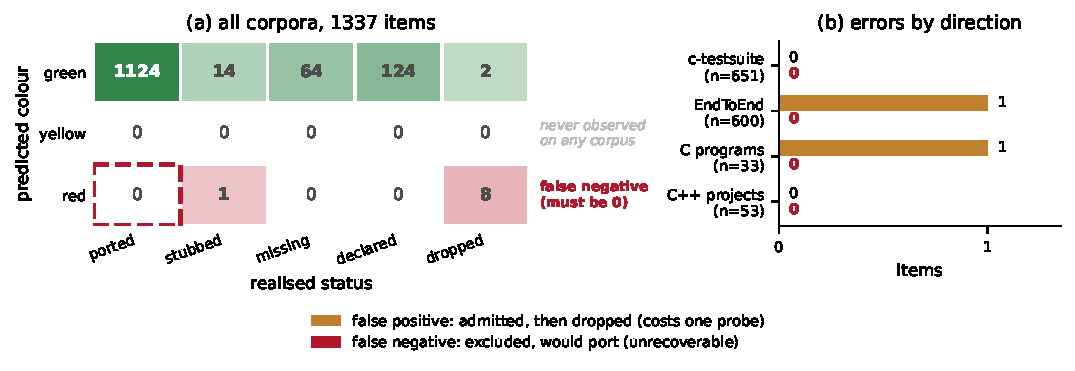
\includegraphics[width=\linewidth]{figures/e1_confusion.pdf}
\caption{Predicted colour against realised item status. The lower-left cell
(predicted \red{red}, realised \texttt{ported}) is the contract-violating
false negative; \S\ref{sec:directional} argues it must be empty.}
\label{fig:e1}
\end{figure}

\subsection{E2: yield of compiling artifacts}
\label{sec:eval-yield}

Table~\ref{tab:e2} and Figure~\ref{fig:e2} report 352 projects. Both columns
count crates that \texttt{cargo build --release} \emph{accepts}, not crates
that were merely written to disk---the distinction matters, because
\S\ref{sec:recovery} describes a bug in which the tool cheerfully emitted
crates that did not compile.

The effect is concentrated exactly where one would predict. On the two
regression corpora, which exist precisely because they are inside the
supported subset, partial translation adds little: c-testsuite is $220/220$
either way. On the demand-signal corpora it is decisive: the C\texttt{++}
projects go from $4/6$ to $6/6$ and the C programs from $9/13$ to
$\mathbf{13/13}$.
Aggregated, $338 \rightarrow 349$ of 352 projects yield a compiling crate.
Excluding c-testsuite, which passes 220/220 under both modes and dilutes every
average, the honest denominator is $n=124$: $116$ (93.5\,\%) under
all-or-nothing against $\mathbf{124}$ ($\mathbf{100\,\%}$) under partial
translation---eight projects converted, and every project in that subset
yielding a compiling crate.

The aggregate understates the case, and we prefer the per-corpus split for
that reason: a benchmark dominated by programs already inside the subset
cannot show much movement, and ours is. The projects that move are the ones
nobody could translate before.

One corpus needs disclosure. The eight \emph{synthetic} projects are our own
constructed test cases, two of which exist specifically to exercise the repair
search. They are reported separately and never folded into a headline, and
where they matter---E3---we say how many of the results are theirs.

\begin{table}[t]
\centering
\footnotesize
\caption{E2: projects yielding a \emph{compiling} Rust crate. ``strict'' is
the conventional all-or-nothing path; ``partial'' is the mode described in
this paper. Both columns count crates that \texttt{cargo build} accepts, not
crates that were merely emitted.}
\label{tab:e2}
\begin{tabular}{@{}lrrrrr@{}}
\toprule
\textbf{corpus} & \textbf{proj.} & \textbf{strict} & \textbf{partial}
 & \textbf{items} & \textbf{\%} \\
\midrule
C\texttt{++} projects & 6 & 4 & \textbf{6} & 40/50 & 80\% \\
C programs & 13 & 9 & \textbf{13} & 18/33 & 55\% \\
EndToEnd & 105 & 103 & \textbf{105} & 457/495 & 92\% \\
c-testsuite & 220 & 220 & \textbf{220} & 609/635 & 96\% \\
synthetic & 8 & 2 & \textbf{5} & 13/20 & 65\% \\
\midrule
total & 352 & 338 & \textbf{349} & 1137/1233 & 92\% \\
\bottomrule
\end{tabular}
\end{table}


\begin{figure}[t]
\centering
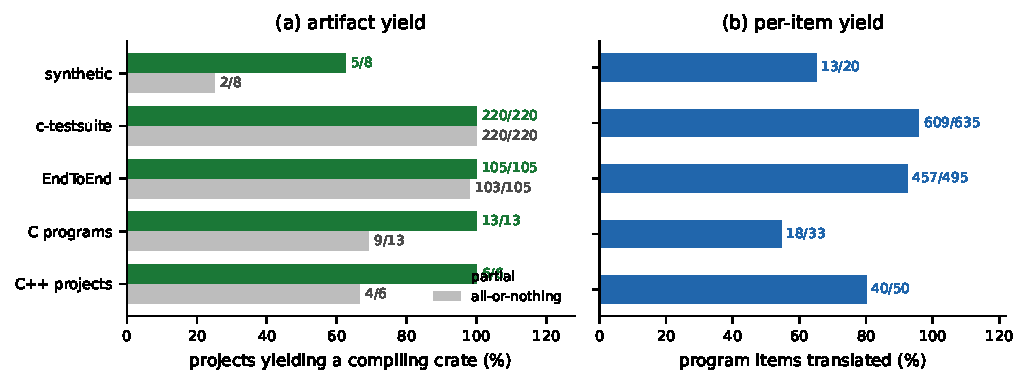
\includegraphics[width=\linewidth]{figures/e2_yield.pdf}
\caption{Projects yielding a compiling Rust crate under all-or-nothing versus
partial translation, and per-item translated fraction.}
\label{fig:e2}
\end{figure}

\subsection{E3: search cost and benefit}
\label{sec:eval-search}

Across all 352 projects, enabling the repair search improves \textbf{3} and
regresses \textbf{none} (Figure~\ref{fig:e3}). All three are
\texttt{test/Project/search-*} fixtures we wrote to exercise the search, each
of which deliberately declares a symbol no translation unit defines. On
non-synthetic input the search improves \textbf{nothing}.

We report this as the paper's central negative result, and we arrived at it by
correcting ourselves. An earlier version of this evaluation reported nine
improvements, six of them pre-existing multi-unit regression tests---and we
cited that provenance as evidence the result was not self-serving. It was an
artifact of our own harness. Those six tests take two translation units, with
the companion source named on the test's own invocation line; the harness
enumerated every case in that directory as a single file and therefore fed
each of them half its source. A symbol that is in fact defined became
undefined, the translation failed for a reason the project did not have, and
the search then ``rescued'' it. We were measuring the search repairing damage
the measurement had done.

The corrected numbers are worse for the mechanism than a simple retraction
would suggest. Given their real inputs all seven affected projects---we found
a seventh the first audit missed---translate under plain all-or-nothing
translation, with no recovery and no search. And on those projects the
search's output had been strictly \emph{worse} than plain translation now
achieves: on one, search yielded 1 of 6 items where strict translation yields
6 of 6. It was withdrawing real, translatable code to route around symbols
the harness had hidden.

\paragraph{What survives.} The guarantee of \S\ref{sec:baseline} survives
intact and is now doing visible work: zero regressions across all 352
projects, including every project whose measurement changed. Cost is
unchanged: median $1.17\times$ wall clock, mean $1.21\times$, p90
$1.40\times$, and 96.0\,\% of projects run a single probe. The budget sweep
still shows every rescue completing at a bound of \textbf{2} while probe
count rises linearly to 16 (Figure~\ref{fig:e3}c), so our shipped default of
8 remains four times larger than anything needs.

\paragraph{What this costs the design.} Contribution~2
(\S\ref{sec:directional}) predicted the search repairs false positives and
whole-program failures. E1 finds two false positives in 1337 items, so the
first role is empirically idle; the second role now has \emph{no}
non-synthetic instance in our benchmark. The error asymmetry we argue for
remains sound as an analysis---and \S\ref{sec:baseline}'s construction is what
makes an idle search harmless rather than harmful---but on this evidence we
cannot claim the search earns its place in the pipeline. It is a mechanism
awaiting a corpus that exhibits the failure mode it addresses, and we now know
that our benchmark does not.

\begin{figure}[t]
\centering
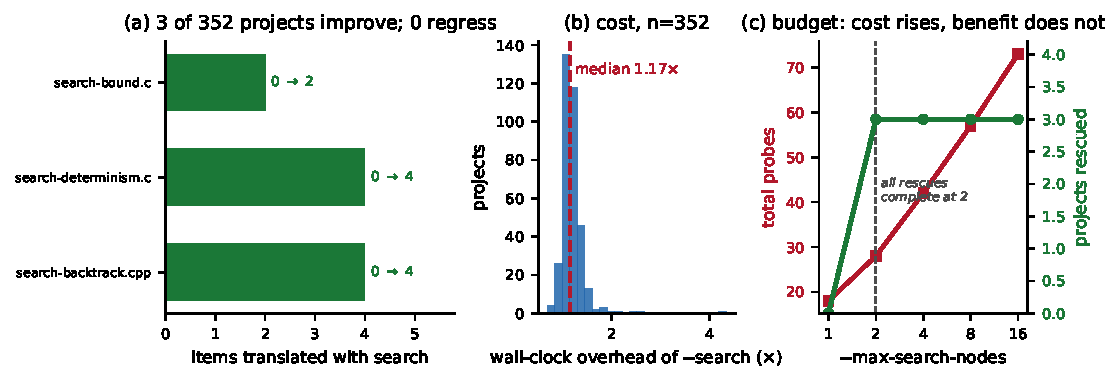
\includegraphics[width=\linewidth]{figures/e3_search.pdf}
\caption{Repair-search benefit and cost. (a) every project the search
improves is a fixture written to exercise it; (b) the cost distribution over
all 352 projects; (c) a budget sweep---probe count rises linearly with the
bound while rescues plateau at 2, so the shipped default of 8 is four times
larger than anything needs.}
\label{fig:e3}
\end{figure}

\subsection{E4: longitudinal progress}
\label{sec:eval-long}

We rebuilt the translator at eight successive revisions and ran each build
against a benchmark frozen from the newest of them---18 projects (13 C, 5
C\texttt{++}), extracted once and never regenerated. Figure~\ref{fig:e4}.

\paragraph{A control isolates the effect.} Because the supported subset also
grew over this period, a rising staircase alone would not show that
\emph{partial translation} caused it. We therefore ran a second series:
all-or-nothing mode at \emph{every} revision, including those that support
partial translation. The control yields $10, 10, 11, 11, 11, 11, 11, 12$
compiling crates; the treatment yields
$10, 10, 11, \mathbf{16}, 16, 16, 16, \mathbf{18}$. The $11 \rightarrow 16$
step is attributable to the mode, not to subset growth, and the final
$16 \rightarrow 18$ to the revision of \S\ref{sec:discussion} that added
library-crate emission. At the last revision \emph{every} project in the
benchmark yields a compiling crate.

\paragraph{Emitted implies compiling.} Across every project-revision
measurement in both series, \texttt{crate\_emitted} and
\texttt{crate\_builds} are identical: no revision ever emitted a crate that
\texttt{cargo} then rejected. This is the invariant of \S\ref{sec:recovery}
holding empirically over the whole history.

\paragraph{Reading the per-item panel.} The lower panel's denominators grow at
the final revision, because two projects that previously produced no report at
all became measurable. The C series moves $18/32 \rightarrow 18/33$---a
\emph{fall} in percentage terms that is not a regression: the extra item is
the \texttt{main} that revision made reportable, and it is unported. This is
the mirror of the usual hazard, and worth stating plainly: on a benchmark
whose membership can change, a rising fraction may be dilution and a falling
one may be honesty. We give both numerator and denominator at every point for
that reason.

\paragraph{Monotonicity.} No project regresses on either series at any
revision, and per-item counts are non-decreasing over the revisions where they
are defined. The visible per-item movement is \texttt{polygon} going
$2/8 \rightarrow 4/8$ at the revision that added C\texttt{++} reference
parameters, and the two projects that begin yielding at the last one.

\paragraph{Reproducibility.} This experiment was run twice, several days
apart, in independent clones, with the seven original revisions rebuilt from
scratch each time. The two runs agree \emph{exactly}, project for project, on
all 119 shared rows of both the treatment and the control series. A per-row
diff over the other five experiments changes only the rows belonging to the
one project whose behaviour genuinely changed between the runs.

\begin{figure}[t]
\centering
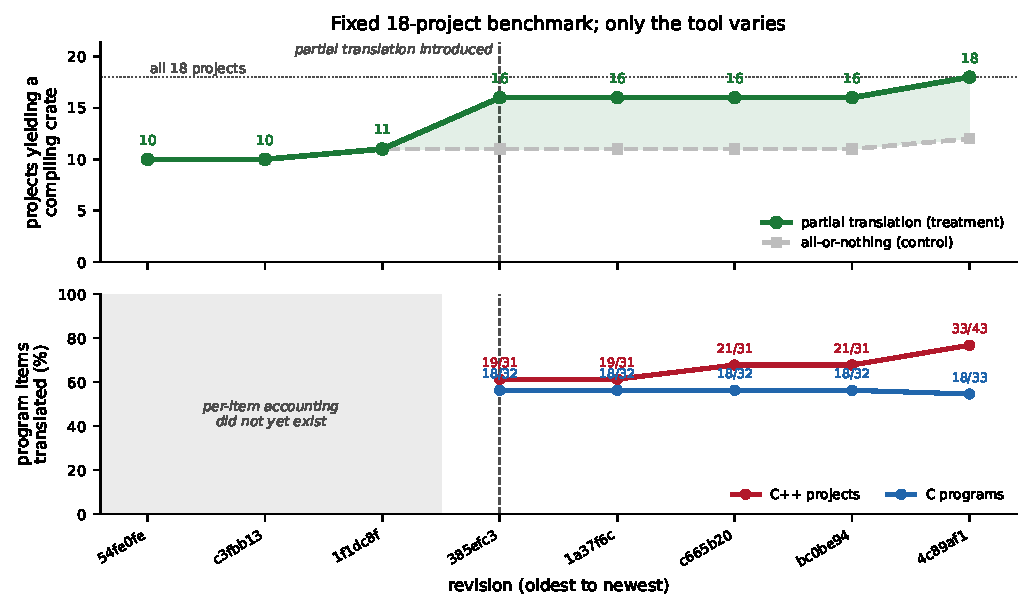
\includegraphics[width=\linewidth]{figures/e4_longitudinal.pdf}
\caption{Translated-item fraction on a fixed benchmark across successive
revisions of the translator.}
\label{fig:e4}
\end{figure}

\subsection{E5: attribution compression}
\label{sec:eval-attrib}

Only eight projects in the measured set reject anything at all, and
attribution is worthwhile in exactly one of them---but that one is the
interesting case. In the \texttt{shapes} project, 19 rejected items carrying
5 distinct direct blocker tags resolve to \textbf{4 root items} under 2 root
tags, a $4.75\times$ compression: thirteen of the nineteen are the identical
``method of an unimported class'', all consequences of one destructor and
three base classes. Across the other seven projects the ratio is exactly
$1.0$---each rejection is its own root, and attribution neither helps nor
hurts. The median compression over all eight is therefore $1.0$ and the
maximum is $4.75$, and the mean over the eight is $1.60$.

We report this shape honestly because it identifies when the mechanism earns
its cost: attribution pays where rejections \emph{cascade}, and cascades
require a language feature that makes many items depend on one declaration.
C\texttt{++} classes do; the C corpora largely do not. A reader porting C
should not expect this to matter, and a reader porting C\texttt{++} should.

\begin{figure}[t]
\centering
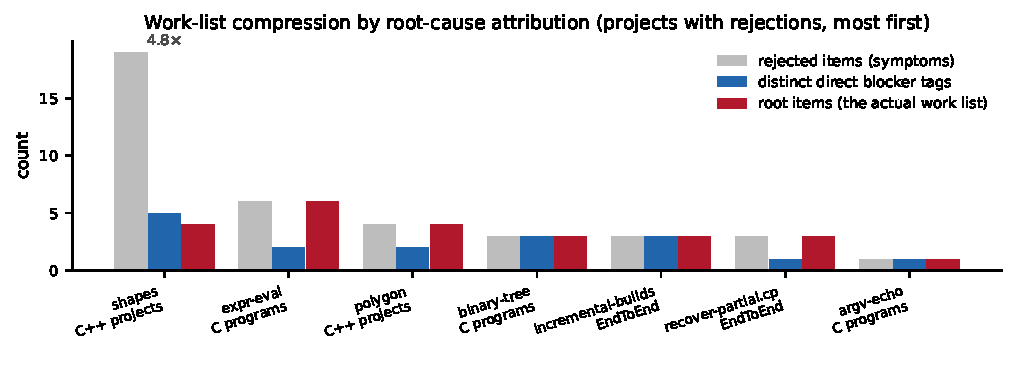
\includegraphics[width=\linewidth]{figures/e5_attribution.pdf}
\caption{Direct blocker tally against root-cause tally.}
\label{fig:e5}
\end{figure}

\subsection{E6: analysis cost}
\label{sec:eval-cost}

We expected the pure-AST analyses to be cheap relative to translation. As
stated, that is \textbf{false}: the item graph costs a median $0.77\times$ a
full translation and the colouring $0.76\times$ (Figure~\ref{fig:e6}). All
three modes pay the same clang parse, which dominates every project in our
benchmark---the median project has two program items, so the analysis proper
is measuring almost nothing.

The claim survives only in the form we should have stated it: \emph{the
analyses do not scale with project structure, and translation does.}
Regressing time on graph size (nodes plus edges), the item graph costs
0.050\,ms per element and the colouring 0.036, against 0.384 for
translation---a $7.6\times$ slope difference. Bucketed by size, the
analysis-to-translation ratio falls from 0.81 on the smallest projects to
\textbf{0.30} at 100 elements and above. A tool should still reuse one parse
across all three modes, as ours does when the search and the report share a
graph.

Operationally the comparison that matters is with the Rust compiler. Summed
over all 352 projects: item graph 11.0\,s, colouring 10.9\,s, translation
15.2\,s, and \texttt{cargo build} \textbf{227.2\,s}---the whole tool is
6.7\,\% of the Rust compiler's time on its own output. The entire
analysis-and-translation pipeline costs an order of magnitude less than
compiling its own output. Analysis cost is not what bounds this workflow.

\begin{figure}[t]
\centering
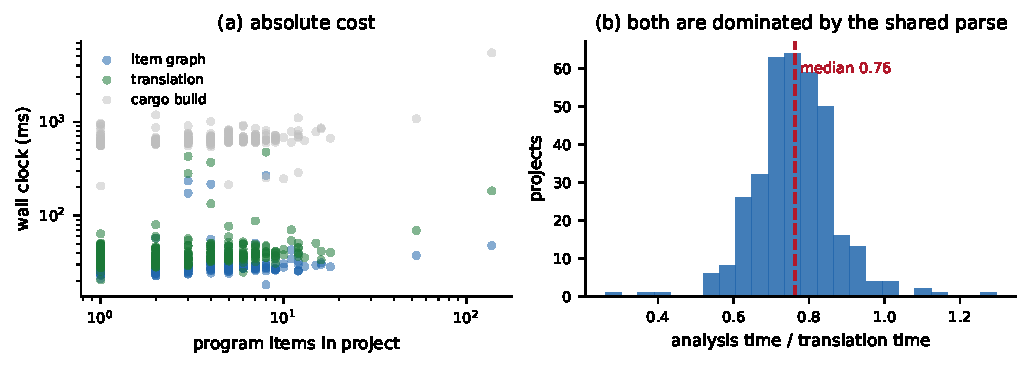
\includegraphics[width=\linewidth]{figures/e6_cost.pdf}
\caption{Pure-AST analysis cost relative to full translation.}
\label{fig:e6}
\end{figure}

\section{Related Work}
\label{sec:related}

\paragraph{C-to-Rust translation.} \textsc{C2Rust} and its predecessor
\textsc{Corrode} translate C to Rust that is faithful but largely
\texttt{unsafe}, on the premise that safety is recovered afterwards by
refactoring. A line of work then attacks that recovery: \textsc{Laertes} drives
raw-pointer elimination with feedback from the Rust borrow checker, and
subsequent ownership analyses infer pointer ownership to guide the same
transformation. Our system differs in target and in failure mode: we emit safe
Rust directly and reject what we cannot, so our problem is not
``unsafe-to-safe'' but ``rejected-to-translated''. Our repair loop resembles
Laertes' compile-and-refine structure, but the signal is our own translator's
per-item rejections rather than \texttt{rustc} diagnostics, and---per
\S\ref{sec:directional}---our loop is subtractive, which is what makes the
error-direction asymmetry load-bearing.

\paragraph{Partial and gradual migration.} The idea of migrating a system
incrementally is old, and foreign-function interfaces are the usual mechanism.
Our stubs are not an FFI boundary: the stub is Rust, has the translated
signature, and is intended to be replaced by hand rather than to call back
into C. The contribution is not partiality itself but the requirement that the
partial artifact \emph{compile}, which is what forces the dependency
discipline of \S\ref{sec:colouring}.

\paragraph{Type qualifier inference and colouring.} Propagating a lattice over
a program graph is standard, from type-qualifier inference onward. What we
believe is new is that our lattice's transfer function is derived from the
\emph{backend's rendering decisions}---the \textsc{Field}/\textsc{FieldIndirect}
split of \S\ref{sec:field-indirect} is invisible in the source type system and
exists only because of how the emitter renders pointers.

\paragraph{Verification-based translation.} An alternative discipline
discharges verification conditions with an SMT solver to certify each
transformation. We considered and rejected this: our soundness evidence is
differential execution against a native build, and where a solver would decide
whether a translation is admissible, we simply attempt it. Attempting is
cheaper here because the translator is the specification, and a solver would
need a second model of it that could drift.

\paragraph{Search-based and repair-driven compilation.} Superoptimisation and
program repair search over candidate programs. Our search is unusual in being
subtractive over an \emph{admission set} rather than generative over program
texts, which is exactly the structure that produces the error asymmetry we
report and the monotonicity guarantee of \S\ref{sec:baseline}.

\section{Discussion and Limitations}
\label{sec:discussion}

Four measurement caveats surfaced during evaluation and materially qualify
the numbers above; we state them rather than let a reader discover them in the
artifact.

\paragraph{Our harness mis-invoked the tool, and the tool got the credit.}
\S\ref{sec:eval-search} describes the defect: seven multi-unit tests were
enumerated as single files, so each was fed half its source, and the repair
search was measured rescuing projects our own measurement had broken. We
record the shape of the mistake because nothing about it is specific to this
system. A harness that mis-invokes the tool under test does not usually
produce an obviously broken number; it produces a plausible one, and it
flatters whatever component recovers from the damage. Ours survived one round
of review, a written argument that its provenance made it trustworthy, and a
re-run of the entire suite at a single commit---because the re-run faithfully
reproduced the same wrong invocation. It was caught only when an unrelated
change made a contradictory claim about the same tests. The general defence we
would now insist on is that a benchmark harness derive its invocation from the
same source of truth the project's own test runner uses, rather than
reimplementing discovery; ours now parses each test's own command line.

\paragraph{The translated fraction is under-reported.} The per-item report
decides that an item was translated by looking up its symbol in the emitted
module. That lookup misses items emitted as \emph{methods} inside an
\texttt{impl} block by our owner-struct model. Auditing all 61 items reported
\texttt{missing}, we found \textbf{24 of them textually present in the crate}.
Every translated-fraction figure in this paper is therefore pessimistic by up
to 24 items corpus-wide. We report the measured numbers unadjusted and flag
the bug; correcting the lookup would move results in our favour, which is
precisely why we did not do it before measuring.

\paragraph{One corpus carries no signal.} All 220 c-testsuite programs
translate completely, contributing 651 items with zero rejections. They
confirm the colouring but cannot discriminate either error direction; the
entire E1 signal comes from the C\texttt{++} projects and the single-file
regression corpus. A reader should weight the headline ratio accordingly.

\paragraph{The guarantee was conditional on the entry point, and the fix
generalised.} An earlier revision of this system emitted only \emph{binary}
crates, so a project whose \texttt{main} was itself dropped yielded no crate
at all---precisely the all-or-nothing behaviour partial translation exists to
remove. Emitting a \emph{library} crate when no \texttt{main} survives closes
it, and the last revision measured here does so: every project in the
longitudinal benchmark now yields a compiling crate.

The episode is worth reporting for what it says about the benchmark rather
than the tool. Library projects---most real C and C\texttt{++} code---were
unreachable under \emph{any} flag, a far larger restriction on the input
surface than any single unsupported construct. Our benchmark could not see it,
because every program in it was authored with a \texttt{main} so that the
differential oracle would have something to run. The blind spot was designed
into the evaluation, not into the translator, and we found it only because a
reader asked why libraries and binaries were not distinguished. Benchmarks
built around an oracle inherit that oracle's preconditions as blind spots; we
know of no general defence beyond saying so.

The fix also forced an honest accounting question. A library that compiles is
weaker evidence than a binary that runs and matches a native build, so the
harness records it as a distinct outcome rather than widening the
differential-verified one. Merging them would have quietly weakened the very
oracle this system's soundness rests on.

The clearest limitation is benchmark scale: four C\texttt{++} projects cannot
establish external validity, and we report them individually for that reason.
A second is that the search's benefit is
concentrated in one failure mode (\S\ref{sec:eval-search}): it rescues
whole-program failures, of which our benchmark contains eight, and repairs
colouring errors, of which it contains two. A corpus without multi-unit
programs would show it earning nothing, and we cannot say which is
representative. A third is that the colouring's contract
is empirical: we argue false negatives must be zero and measure that they are,
but we do not prove it, and the one deliberately-retained false negative
(a body dependency reached through a pointer) is admitted because the
baseline-state construction recovers it.

The transferable claims, in our view, are the three design rules. Any system
that generates code in a target language and must tolerate partial failure
faces the substitutability question of \S\ref{sec:colouring}. Any system that
pairs a static approximation with a subtractive search faces the error
asymmetry of \S\ref{sec:directional}. Any system whose search can degrade its
input should make the input a search state, as in \S\ref{sec:baseline}. None
of the three is specific to Rust or to C\texttt{++}.

\section*{Artifact}

All measurements report a \emph{single} revision of the translator, taken in
a clean checkout with an empty working tree before and after; the longitudinal
experiment is the sole exception and varies the revision by construction. An
earlier draft of this paper mixed two revisions across its experiments, which
is exactly the defect that makes a results table unfalsifiable, so the entire
suite was re-run rather than patched.

Every number and every figure in this paper is generated from measurement CSVs
by two scripts (\texttt{scripts/tables.py}, \texttt{scripts/plots.py}); none is
transcribed by hand. The harnesses that produced the CSVs, the frozen E4
benchmark with the commit it was extracted from, and the raw per-invocation
records are included alongside. E1 measured all 340 candidate projects with no
sampling; the seven that produced no per-item report are listed with reasons
rather than omitted.

\section{Conclusion}

Making partial output the deliverable changes what an incomplete translator is
worth: it turns a wall of diagnostics into a compiling artifact with a ranked
work list, and it turns ``how far along are we'' into a number one can plot.
The three decisions that made it work---edge semantics derived from the
emitter, approximation deliberately unsound in the recoverable direction, and
the trivial solution as a member of the search space---were each forced on us
by a measurement that contradicted a specification we had written. We report
them, and the measurement that contradicted each, in the hope that the next
system does not have to be corrected the same way.

\end{document}
